\chapter{沉淀与溶解度}\label{ch:b1:precipitation}

一滴硝酸银滴入自来水，随即出现一片白色浑浊：
氯化银沉淀，它由每升水中仅有的几毫克氯离子
生成。渗过石灰岩的水将碳酸钙带走，
又将其沉积下来，每年仅几分之一毫米，
形成洞穴中的钟乳石与石笋。肾结石也是一种沉淀。这些现象
都是固体与其溶液中离子间的平衡，其中有一个
常数，即溶度积，可说明固体是否生成、
溶解多少，以及另一种离子或 pH 改变时
溶解度如何变化。借助它，化学家可以
通过依次沉淀离子而将其逐一分开——这正是
本章末尾矿井水处理的基础。

\begin{recall}
第 1 册（六年级与十二年级）以克每升表示溶解度，
并依据离子所生成的沉淀来鉴别离子。平衡
常数、反应商 $Q$ 与活度（纯固体或溶剂为 1，
溶质为 $c/c^\circ$），这些均
在\cref{ch:b1:extent-q-and-k}中建立：当 $Q < K$ 时反应正向进行。
主反应方法与 $\mathrm{p}K_a$ 标度，
见\cref{ch:b1:predominant-reaction}；$c^\circ = \qty{1}{mol/L}$ 不
写入商中。
\end{recall}

\begin{omfigure}
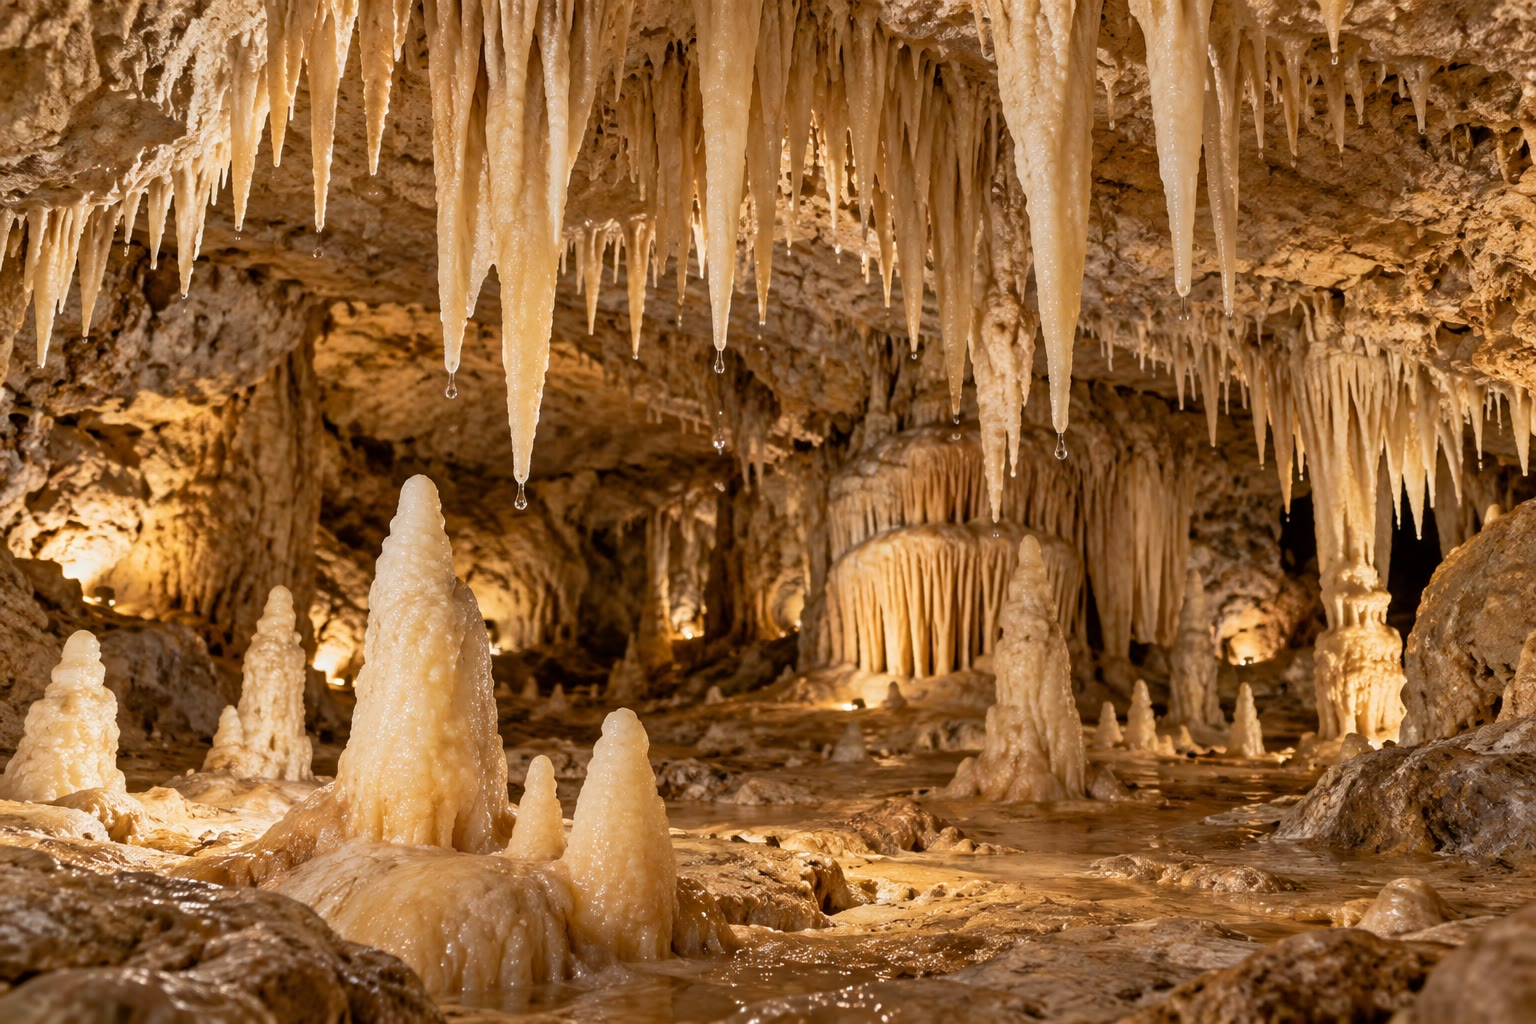
\includegraphics[width=0.62\linewidth]{images/book2/ai/b1-11-cave.jpg}

{\small 石灰岩洞穴中的钟乳石与石笋。富含二氧化碳的水
溶解上方土壤中的碳酸钙；在洞穴中，
水失去部分二氧化碳，碳酸盐重新沉淀，
（见\cref{exo:b1:precipitation:10}）。}
\end{omfigure}

\section{溶度积}\label{sec:b1:precipitation:product}

投入水中的一粒氯化银晶体向溶液失去离子，
溶液又将部分离子返还给晶体。当两者
速率相等时，溶液处于\emph{饱和}状态：其组成不再
改变，但离子仍在两个方向上不断迁移
（见下图）。

\begin{definition}[溶度积]\label{def:b1:precipitation:solubility-product}
称\emph{溶度积}\index{溶度积} $K_s$ 为离子型
固体 $\mathrm{M}_a\mathrm{X}_b$ 溶解为离子的
平衡常数，
\[
  \mathrm{M}_a\mathrm{X}_b\mathrm{(s)} \rightleftharpoons a\,\mathrm{M}^{m+}
  + b\,\mathrm{X}^{x-}, \qquad
  K_s = [\mathrm{M}^{m+}]_{\mathrm{eq}}^{\,a}\,[\mathrm{X}^{x-}]_{\mathrm{eq}}^{\,b},
  \qquad \mathrm{p}K_s = -\log K_s ,
\]
固体的活度为 1。与所有平衡常数一样，它
只依赖于温度。
\end{definition}

对于氯化银，\ce{AgCl(s) <=> Ag+ + Cl-}，且 $K_s =
[\ce{Ag+}][\ce{Cl-}] = 10^{-9.75}$；对于氟化钙，\ce{CaF2(s) <=>
Ca^2+ + 2F-}，且 $K_s = [\ce{Ca^2+}][\ce{F-}]^2 = 10^{-9.84}$；对于
氢氧化铁（III），$K_s = [\ce{Fe^3+}][\ce{OH-}]^3 = 10^{-38.55}$。
下表列出了本册所用的数值。
它们与 $\mathrm{p}K_a$ 的算法相同（见
\cref{ch:b1:predominant-reaction}），由列表给出的标准吉布斯
生成自由能计算得出：$\mathrm{p}K_s = \Delta_r G^\circ/(RT\ln 10)$，此关系式
在本科二年级分册中推出。

\begin{omfigure}
\begin{tikzpicture}[font=\small, >={Stealth}]
  % the crystal: alternating Ag+ (small, grey) and Cl- (large, green)
  \foreach \i in {0,1,2,3,4,5}
    \foreach \j in {0,1,2} {
      \pgfmathtruncatemacro{\pp}{mod(\i+\j,2)}
      \ifnum\pp=0
        \shade[ball color=green!55!black!60] (\i*0.62,\j*0.62) circle (0.29);
      \else
        \shade[ball color=gray!35] (\i*0.62,\j*0.62) circle (0.17);
      \fi }
  \draw[thick, gray] (-0.45,-0.45) rectangle (3.55,1.75);
  \node[below] at (1.55,-0.45) {氯化银 \ce{AgCl(s)}};
  % ions in solution
  \shade[ball color=gray!35] (1.2,3.0) circle (0.17);
  \node[right] at (1.4,3.0) {\ce{Ag+}};
  \shade[ball color=green!55!black!60] (2.6,2.7) circle (0.29);
  \node[right] at (2.9,2.7) {\ce{Cl-}};
  \shade[ball color=gray!35] (4.4,1.4) circle (0.17);
  \shade[ball color=green!55!black!60] (5.1,2.6) circle (0.29);
  \shade[ball color=gray!35] (-1.0,2.4) circle (0.17);
  \shade[ball color=green!55!black!60] (-0.6,3.3) circle (0.29);
  % arrows: dissolution and precipitation
  \draw[->, thick, omDef] (1.24,1.6) to[bend left=20] node[left, pos=0.6] {溶解} (1.15,2.78);
  \draw[->, thick, omProp] (2.55,2.38) to[bend left=20] node[right, pos=0.45] {沉淀} (2.45,1.55);
  % the water line
  \draw[blue!50, thick] (-1.6,3.8) -- (5.9,3.8);
  \node[blue!60!black, anchor=east] at (5.9,4.05) {饱和溶液};
\end{tikzpicture}

{\small 氯化银晶体置于其饱和溶液中。离子
从表面离开（溶解），另有离子被捕获（沉淀），两者
以相同速率进行，使 $[\ce{Ag+}][\ce{Cl-}]$ 保持等于 $K_s$。银离子
图中银离子画得比氯离子小，与实际相符。}
\end{omfigure}

\begin{omfigure}
\begin{tabular}{lc@{\qquad}lc}
\hline
固体 & $\mathrm{p}K_s$ & 固体 & $\mathrm{p}K_s$ \\
\hline
\ce{AgCl} & 9.75 & \ce{Ca(OH)2} & 5.33 \\
\ce{AgBr} & 12.27 & \ce{Mg(OH)2} & 11.25 \\
\ce{AgI} & 16.07 & \ce{Fe(OH)2} & 16.31 \\
\ce{Ag2CrO4} & 11.95 & \ce{Zn(OH)2} & 16.38 \\
\ce{BaSO4} & 9.97 & \ce{Fe(OH)3} & 38.55 \\
\ce{CaCO3}（方解石） & 8.30 & \ce{Al(OH)3}（三水铝石） & 34.75 \\
\ce{CaF2} & 9.84 & & \\
\hline
\end{tabular}

\smallskip
{\small 溶度积数据为 \qty{25}{\celsius} 下的值，由
固体及水合离子的标准吉布斯生成能计算得出。
本章所用的形成常数（见\cref{sec:b1:precipitation:amphoteric}）：
$\log\beta_4 = 14.45$ 对应 \ce{Zn(OH)4^2-}，33.52 对应 \ce{Al(OH)4-}，以及
$\log\beta_1 = 11.82$ 对应 \ce{FeOH^2+}。}
% ledger: dfg:AgCl_cr, dfg:AgBr_cr, dfg:AgI_cr, dfg:Ag2CrO4_cr, dfg:Ag+_ao, dfg:Cl-_ao, dfg:Br-_ao, dfg:I-_ao, dfg:CrO42-_ao (computed in figdata/bachelor-1/aqueous-constants.py)
% ledger: dfg:BaSO4_cr, dfg:Ba2+_ao, dfg:SO42-_ao, dfg:CaCO3_cr, dfg:CO32-_ao, dfg:CaF2_cr, dfg:Ca2+_ao, dfg:F-_ao (computed, same script)
% ledger: dfg:Ca_OH2_cr, dfg:Mg_OH2_cr, dfg:Mg2+_ao, dfg:Fe_OH2_cr, dfg:Fe2+_ao, dfg:Zn_OH2_cr, dfg:Zn2+_ao, dfg:Fe_OH3_cr, dfg:Fe3+_ao, dfg:Al2O3.3H2O_cr, dfg:Al3+_ao, dfg:OH-_ao (computed, same script)
% ledger: dfg:Zn_OH42-_ao, dfg:Al_OH4-_ao, dfg:FeOH2+_ao (formation constants, same script)
\end{omfigure}

\begin{proposition}[沉淀条件]\label{prop:b1:precipitation:precipitation-condition}
设溶液含有固体 $\mathrm{M}_a\mathrm{X}_b$ 的离子，
反应商 $Q_s = [\mathrm{M}^{m+}]^a[\mathrm{X}^{x-}]^b$ 用于
描述溶解过程。
\begin{itemize}
  \item 若 $Q_s < K_s$，则固体不可能在平衡时存在：
        溶液未饱和，加入的任何固体都会溶解，
        若固体量不太多则完全溶解。
  \item 若 $Q_s > K_s$，则固体沉淀，直至 $Q_s = K_s$。
  \item 固体与溶液在平衡时共存，仅当
        $Q_s = K_s$。
\end{itemize}
\end{proposition}

\begin{proof}
由\cref{ch:b1:extent-q-and-k}可知，只要
$Q_s < K_s$，溶解正向进行；只要 $Q_s > K_s$，则逆向进行（沉淀）。溶解正向进行时，
$Q_s$ 增大。若固体在
$Q_s$ 达到 $K_s$ 之前已耗尽，则反应停止，体系中不再有固体：纯凝聚相参与的反应
可能在达到平衡前停止，因为该相的物质的量不能为负。
若 $Q_s > K_s$，沉淀使
两种离子浓度均下降，$Q_s$ 随之减小，直至等于 $K_s$，
这总是可以实现的，因为溶液中有离子存在。
\end{proof}

最后一点正是固体与溶解物种的区别所在。一种酸碱物种
在任何 pH 下都存在，无论量多少；而固体
要么存在，要么不存在。因此其图应为
\emph{存在区域}图，而非优势区域图
（见\cref{sec:b1:precipitation:domains}）。

\begin{example}[混合两种溶液]\label{ex:b1:precipitation:mixing}
\qty{10.0}{mL} 浓度为 \qty{2.0e-4}{mol/L} 的硝酸银溶液与
\qty{10.0}{mL} 浓度为 \qty{2.0e-4}{mol/L} 的氯化钠溶液混合。刚混合后
尚未发生反应，$[\ce{Ag+}] = [\ce{Cl-}] = \qty{1.0e-4}{mol/L}$
且 $Q_s = 10^{-8.0} > K_s = 10^{-9.75}$：氯化银沉淀。
若两溶液浓度均为 \qty{2.0e-6}{mol/L}，则 $Q_s = 10^{-12.0} < K_s$，
混合物保持澄清。硝酸银是检验氯
离子的灵敏试剂，但并非无限灵敏。
\end{example}

\begin{inthelab}[氯离子检验]
在教学实验室中，向样品中滴加数滴硝酸银溶液，
样品事先用稀硝酸酸化。硝酸
可将碳酸根与氢氧根离子转化为二氧化碳和水，这些离子若不除去，
也会与银离子一同沉淀。白色沉淀
见光变暗的即为氯化银；溴化物给出米黄色
沉淀，碘化物则给出黄色沉淀
（见下图）。
硝酸银会使皮肤染黑：须佩戴手套和护目镜。
\end{inthelab}

\begin{omfigure}
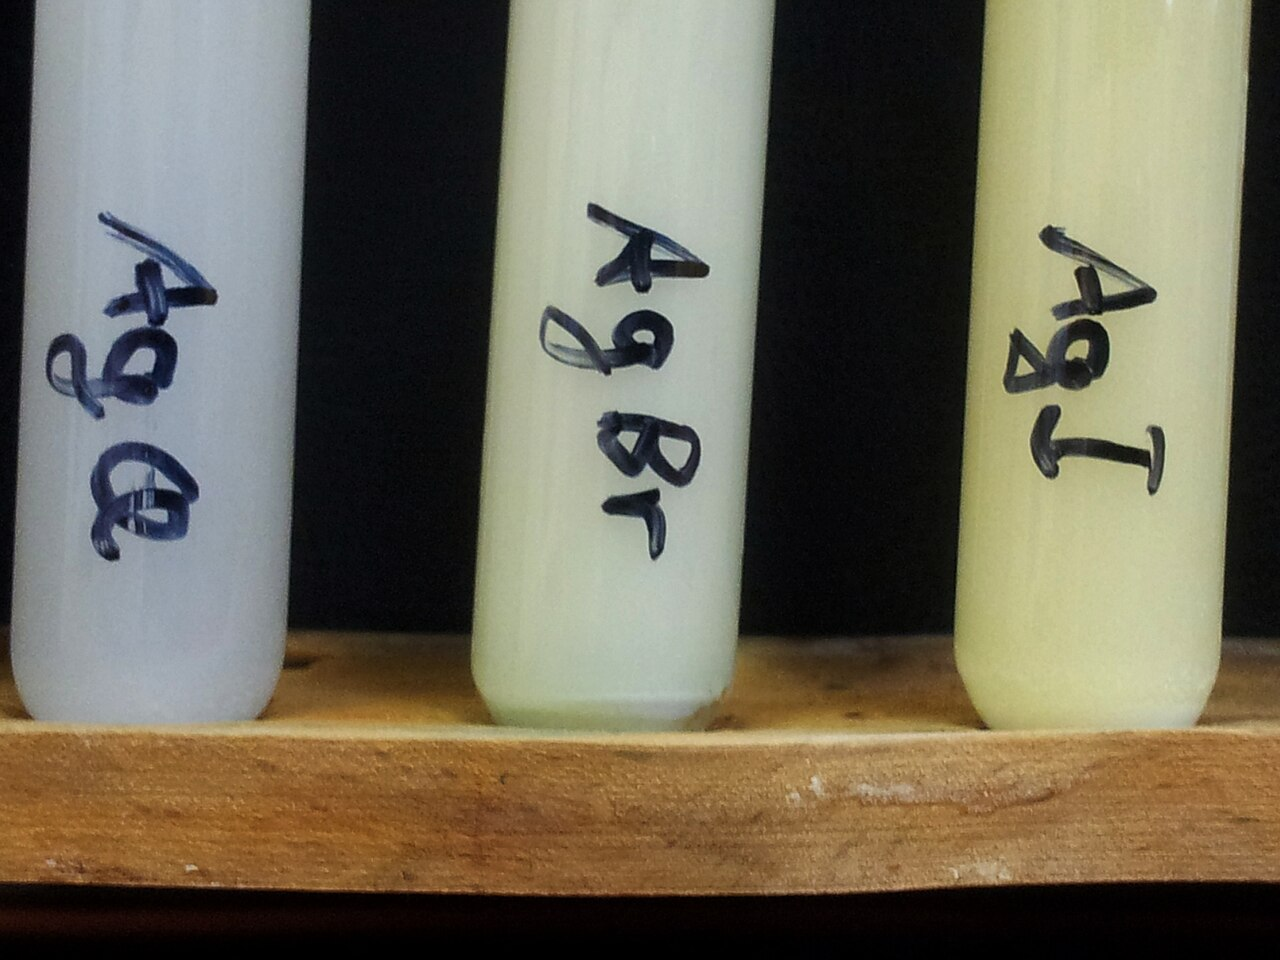
\includegraphics[width=0.6\linewidth]{images/book2/silver-halides.jpg}

{\small 氯化银（白色）、溴化银（米黄色）
和碘化银（浅黄色）的沉淀。
照片：Rrausch1974，CC BY-SA 3.0，维基共享资源。}
\end{omfigure}

\section{溶解度}

\begin{definition}[溶解度]\label{def:b1:precipitation:solubility}
称固体在给定溶液中的\emph{溶解度}\index{溶解度} $s$
为一升该溶液中溶解至饱和时溶解的固体量（以 \unit{mol/L} 计）；
乘以摩尔质量后，即得质量溶解度，
单位为 \unit{g/L}。它与温度
及溶液的组成有关。
\end{definition}

\begin{proposition}[由溶度积求溶解度]\label{prop:b1:precipitation:s-of-ks}
在纯水中，若离子不参与其他反应，
\[
  \mathrm{MX}:\ s = \sqrt{K_s}, \qquad
  \mathrm{MX_2}\ \text{或}\ \mathrm{M_2X}:\ s = \left(\frac{K_s}{4}\right)^{1/3},
  \qquad
  \mathrm{M}_a\mathrm{X}_b:\ s = \left(\frac{K_s}{a^a b^b}\right)^{1/(a+b)} .
\]
\end{proposition}

\begin{proof}
每升溶解 $s$ 摩尔固体时，$[\mathrm{M}^{m+}] = as$，且
$[\mathrm{X}^{x-}] = bs$，故饱和时 $K_s = (as)^a(bs)^b =
a^a b^b s^{a+b}$。对于 MX，$a = b = 1$；对于 \ce{MX2}，$1^1 2^2 = 4$，且
\ce{M2X} 的情形相同。
\end{proof}

\begin{example}[氯化银与铬酸银]\label{ex:b1:precipitation:agcl-ag2cro4}
氯化银：$s = 10^{-9.75/2} = \qty{1.3e-5}{mol/L}$，或
\qty{1.9}{mg/L}，其中 $M = \qty{143.4}{g/mol}$。铬酸银 \ce{Ag2CrO4}
（$\mathrm{p}K_s = 11.95$）：$s = (10^{-11.95}/4)^{1/3} =
\qty{6.6e-5}{mol/L}$。铬酸银的 $K_s$ 较小，而其
溶解度却高出五倍。溶度积仅可在
化学式类型相同的固体之间直接比较。
\end{example}

\begin{remark}
公式假定离子是自由的。在纯水中，铬酸根
是弱碱，银离子不与任何物质络合，因此
铬酸银的结果接近正确；对于碳酸盐、
硫化物或氢氧化物，阴离子的碱性起作用，于是
需要下一节的内容。在高离子强度下，活度也会偏离
浓度，这一修正留给本科二年级分册。
\end{remark}

\section{同离子效应与 pH 效应}

\begin{definition}[同离子效应]\label{def:b1:precipitation:common-ion}
称\emph{同离子效应}\index{同离子效应}为固体在
已含有其某一离子的溶液中
溶解度的降低。
\end{definition}

\begin{proposition}[含同离子时的溶解度]\label{prop:b1:precipitation:common-ion}
设 MX 溶于已有 $[\mathrm{X}^-] = c$ 的溶液中，
其中 $c \gg \sqrt{K_s}$。则 $s \approx K_s/c$，远小于
对于 \ce{MX2}，若溶液中 \ce{M^2+} 的浓度为 $c$，
则 $s \approx \frac12\sqrt{K_s/c}$。
\end{proposition}

\begin{proof}
饱和时 $[\mathrm{M}^+] = s$，$[\mathrm{X}^-] = c + s$，于是
$s(c + s) = K_s$。若 $s \ll c$，则 $s = K_s/c$；该假设成立，因为
$K_s/c \ll c$，当 $c^2 \gg K_s$ 时。对于 \ce{MX2}，$[\ce{X-}] = 2s$，且
$[\mathrm{M}^{2+}] = c + s \approx c$，于是 $c\,(2s)^2 = K_s$。
\end{proof}

氯化银在 \qty{0.10}{mol/L} 的氯化钠溶液中：$s = 10^{-9.75}/0.10
= \qty{1.8e-9}{mol/L}$，比在水中的溶解度小七千倍。
这正是沉淀要用同离子的稀溶液而不用纯水
洗涤的原因：它自身损失得更少。

当固体的阴离子是碱时，酸会把它从溶解平衡中拉出，
溶解度随之升高。对于碳酸钙在酸中的溶解，
其反应为
\[
  \ce{CaCO3(s) + H3O+ <=> Ca^2+ + HCO3- + H2O}, \qquad
  K = \frac{K_s}{K_{a2}} = 10^{-8.30 + 10.33} = 10^{2.03} ,
\]
这是一个有利的反应：醋或盐酸能溶解石灰石，
而 \ce{HCO3-} 进一步反应生成的二氧化碳
产生人们熟悉的气泡。
% ledger: dfg:HCO3-_ao (pKa2 of carbonic acid, ch. 10)

\begin{proposition}[氢氧化物的溶解度随 pH 的变化]\label{prop:b1:precipitation:hydroxide-ph}
在给定 pH 的缓冲溶液中，\ce{M^{n+}} 的浓度
与氢氧化物 \ce{M(OH)_n} 平衡时满足
\[
  \log[\mathrm{M}^{n+}] = -\mathrm{p}K_s + n\,(\mathrm{p}K_e - \mathrm{pH}) ,
\]
对 pH 作图为斜率 $-n$ 的直线。若该离子不形成配合物，
则上式即为氢氧化物的溶解度。
\end{proposition}

\begin{proof}
$K_s = [\mathrm{M}^{n+}][\ce{OH-}]^n$，且 $[\ce{OH-}] = K_e/[\ce{H3O+}]$，
于是 $\log[\mathrm{M}^{n+}] = \log K_s - n\log[\ce{OH-}] = -\mathrm{p}K_s -
n(\mathrm{pH} - \mathrm{p}K_e)$。
\end{proof}

pH 每增加一个单位，氢氧化铁（III）的溶解度降为原来的千分之一，
氢氧化锌则降为原来的百分之一。氢氧化物可通过
改变 pH 而沉淀，也可重新溶解。

\begin{example}[用二氧化碳溶解碳酸钙]\label{ex:b1:precipitation:cave}
溶有二氧化碳的水能溶解方解石：
\[
  \ce{CaCO3(s) + CO2(aq) + H2O <=> Ca^2+ + 2HCO3-}, \qquad
  K = \frac{K_s K_{a1}}{K_{a2}} = 10^{-8.30 - 6.37 + 10.33} = 10^{-4.34} ,
\]
该常数由碳酸盐的溶解、二氧化碳的第一步离解，
以及第二步离解的逆过程相加得到。
二氧化碳越多，碳酸钙溶解得越多。土壤空气通常
远比洞穴空气富含二氧化碳；渗过土壤并
到达洞穴顶部的水会失去二氧化碳，并
使方解石沉积（见\cref{exo:b1:precipitation:10}）。
\end{example}

\section{存在区域与选择性沉淀}\label{sec:b1:precipitation:domains}

\begin{definition}[存在区域]\label{def:b1:precipitation:existence-domain}
对于某固体及其一种离子的给定总浓度 $c$，
该固体的\emph{存在区域}\index{存在区域}为
平衡时固体存在的变量（pX、pM 或 pH）的取值范围。其边界为
首次出现固体颗粒时的数值，
即 $Q_s = K_s$ 且该离子浓度仍为 $c$ 时的数值。
\end{definition}

\begin{method}[绘制存在区域图]\label{met:b1:precipitation:existence-domain}
\begin{enumerate}
  \item 固定不在坐标轴上的离子的总浓度 $c$
        （例如在 pCl 坐标轴上取 $[\ce{Ag+}]_{\mathrm{tot}} = c$）。
  \item 在开始沉淀时写出 $K_s$，此时该离子浓度仍为
        $c$，并解出坐标轴上的变量。
  \item 固体存在于另一离子浓度较高的一侧：
        即 pCl 较小（氯离子较多）、pAg 较小，
        或对氢氧化物而言 pH 较高。
  \item 不要为该离子本身标注区域，它处处存在，
        在固体存在区域之外浓度为 $c$，
        在其内部则低于 $c$。
\end{enumerate}
\end{method}

对于氯化银，取 $c = [\ce{Ag+}]_{\mathrm{tot}} = 10^{-2}$：
当 $[\ce{Cl-}] = K_s/c = 10^{-7.75}$ 时开始沉淀，因此固体
存在于 $\mathrm{pCl} < 7.75$ 的范围内。对于碘化银，其边界位于
$\mathrm{pI} = 16.07 - 2 = 14.07$，如下图所示。

\begin{omfigure}
\begin{tikzpicture}[font=\small, >={Stealth}, x=0.62cm]
  \fill[omDef!18] (0,0.12) rectangle (7.75,0.6);
  \draw[->, thick] (0,0) -- (17.2,0) node[right] {pCl 或 pI};
  \foreach \x in {0,2,4,6,8,10,12,14,16}
    \draw (\x,0.08) -- (\x,-0.08) node[below] {\x};
  \draw[omDef, thick] (7.75,-0.5) -- (7.75,0.9);
  \node[omDef] at (3.9,0.36) {\ce{AgCl(s)} 存在};
  \node[omDef, above] at (7.75,0.9) {7.75};
  \node[anchor=west] at (8.0,0.36) {无固体：\ce{Ag+} 浓度 $10^{-2}$ mol/L};
  % AgI below
  \begin{scope}[yshift=-1.9cm]
  \fill[omProp!20] (0,0.12) rectangle (14.07,0.6);
  \draw[->, thick] (0,0) -- (17.2,0);
  \foreach \x in {0,2,4,6,8,10,12,14,16}
    \draw (\x,0.08) -- (\x,-0.08) node[below] {\x};
  \draw[omProp, thick] (14.07,-0.5) -- (14.07,0.9);
  \node[omProp] at (7.0,0.36) {\ce{AgI(s)} 存在};
  \node[omProp, above] at (14.07,0.9) {14.07};
  \end{scope}
\end{tikzpicture}

{\small 氯化银（在 pCl 轴上，上方）与
碘化银（在 pI 轴上，下方）在银总浓度为
\qty{1.0e-2}{mol/L} 时的存在区域。碘离子使银沉淀所需的
浓度比氯离子低百万倍。}
\end{omfigure}

\begin{method}[选择性沉淀]\label{met:b1:precipitation:selective}
要分离两种能与同一试剂生成沉淀的离子：
\begin{enumerate}
  \item 对每种离子，按其浓度计算其固体开始生成时的试剂
        浓度（或 pH）；
        所需浓度较低者先沉淀；
  \item 计算第二种离子开始沉淀时溶液中
        残留的第一种离子的浓度；
  \item 若该浓度足够小，即为初始浓度的一小部分——
        通常为 \qty{0.1}{\percent}——，则分离合格，
        且随后在两个阈值之间停止加入试剂。
\end{enumerate}
\end{method}

\begin{example}[碘离子与氯离子]\label{ex:b1:precipitation:i-cl}
某溶液中含有碘离子和氯离子，两者浓度均为
\qty{1.0e-2}{mol/L}；逐滴加入硝酸银，
且不稀释。碘化银在 $[\ce{Ag+}] = 10^{-16.07 + 2} =
10^{-14.07}$ 时开始生成，氯化银则在 $10^{-9.75 + 2} = 10^{-7.75}$ 时开始生成：碘离子
先沉淀。氯化银出现时，
$[\ce{I-}] = 10^{-16.07}/10^{-7.75} = 10^{-8.32} = \qty{4.8e-9}{mol/L}$，
此时碘离子的剩余分数为 $5 \times 10^{-7}$，分离完全。
\end{example}

氢氧化物可以用同样的方法分离，只是以 pH 作为变量。
下图给出了六种离子在
\qty{0.010}{mol/L} 时，氢氧化物出现时的 pH 以及
\qty{99.9}{\percent} 的离子已沉淀时的 pH。铁（III）与铝
在酸性水中除去，锌与铁（II）在接近中性时除去，镁
在 pH 约为 10 时除去，钙只在很强的碱性水中除去。

\begin{omfigure}
\begin{tikzpicture}
\begin{axis}[
  width=0.82\linewidth, height=5.4cm, xmin=0, xmax=14, ymin=0.4, ymax=6.6,
  axis x line=bottom, axis y line=left, xlabel={pH},
  xtick={0,2,4,6,8,10,12,14}, ytick={1,2,3,4,5,6},
  yticklabels={\ce{Fe^3+}, \ce{Al^3+}, \ce{Zn^2+}, \ce{Fe^2+}, \ce{Mg^2+}, \ce{Ca^2+}},
  y dir=reverse, axis line style={-},
  tick label style={font=\small}, label style={font=\small}]
\addplot[draw=none, omDef!35,
  error bars/.cd, x dir=plus, x explicit,
  error bar style={line width=7pt, omDef!35}, error mark=none]
  table[x=start, y=row, x error expr=14-\thisrow{start}] {figdata/out/bachelor-1-solubility-ph-thresholds.dat};
\addplot[draw=none, omDef,
  error bars/.cd, x dir=plus, x explicit,
  error bar style={line width=7pt, omDef}, error mark=none]
  table[x=start, y=row, x error expr=\thisrow{end}-\thisrow{start}] {figdata/out/bachelor-1-solubility-ph-thresholds.dat};
\end{axis}
\end{tikzpicture}

{\small 溶液中氢氧化物的沉淀，各离子的浓度均为 \qty{0.010}{mol/L}。
深色条带从氢氧化物出现第一粒晶体的 pH 延伸至
\qty{99.9}{\percent} 的离子已沉淀时的 pH（三价离子的条带宽为一个 pH 单位，
二价离子为一点五个 pH 单位）；浅色条带为氢氧化物存在区域的
其余部分。锌和铝的两性氢氧化物在高 pH 下的
再溶解
（见\cref{sec:b1:precipitation:amphoteric}）未在图中示出。}
\end{omfigure}

\section{两性氢氧化物}\label{sec:b1:precipitation:amphoteric}

向硫酸锌溶液中逐滴加入氢氧化钠，生成白色
氢氧化锌沉淀，随后在过量氢氧根中它又
溶解。氢氧化铝的情形相同；氢氧化铁（III）和
氢氧化镁则不会。

\begin{definition}[两性氢氧化物]\label{def:b1:precipitation:amphoteric-hydroxide}
若一种氢氧化物既能在酸中以阳离子形式溶解，又能在过量碱中
以羟基配阴离子形式溶解，则称其为\emph{两性氢氧化物}\index{两性氢氧化物}，
其反应式为：
\[
  \ce{Zn(OH)2(s) + 2H3O+ -> Zn^2+ + 4H2O}, \qquad
  \ce{Zn(OH)2(s) + 2OH- -> Zn(OH)4^2-} .
\]
\end{definition}

配阴离子 \ce{Zn(OH)4^2-}（四羟基合锌酸根）的特征在于其生成常数
$\beta_4 = [\ce{Zn(OH)4^2-}]/([\ce{Zn^2+}][\ce{OH-}]^4)
= 10^{14.45}$；配合物及其常数见
\cref{ch:b1:complexation}。

\begin{proposition}[两性氢氧化物的溶解度]\label{prop:b1:precipitation:amphoteric}
若锌在溶液中仅以 \ce{Zn^2+} 和 \ce{Zn(OH)4^2-} 形式存在，则
氢氧化锌的溶解度为
\[
  s = [\ce{Zn^2+}] + [\ce{Zn(OH)4^2-}] = \frac{K_s}{[\ce{OH-}]^2} + K\,[\ce{OH-}]^2,
  \qquad K = \beta_4 K_s = 10^{-1.93} .
\]
以 $\log s$ 对 pH 作图时，低 pH 下为斜率 $-2$ 的直线，
高 pH 下为斜率 $+2$ 的直线。溶解度最小处满足
$[\ce{OH-}]^4 = K_s/K = 1/\beta_4$，即 $\mathrm{pH} =
\mathrm{p}K_e - \frac14\log\beta_4$，此时 $s_{\min} = 2\sqrt{K_s K}$。
\end{proposition}

\begin{proof}
饱和时 $[\ce{Zn^2+}] = K_s/[\ce{OH-}]^2$，且
$[\ce{Zn(OH)4^2-}] = \beta_4[\ce{Zn^2+}][\ce{OH-}]^4 = \beta_4 K_s
[\ce{OH-}]^2$。令 $w = [\ce{OH-}]^2$，则 $s(w) = K_s/w + Kw$ 的导数为
$-K_s/w^2 + K$，在 $w = \sqrt{K_s/K}$ 处为零，此时 $s = 2\sqrt{K_s K}$。
在低 pH 时第一项占主导，$\log s = \log K_s - 2\log[\ce{OH-}]$
（对 pH 的斜率为 $-2$）；在高 pH 时第二项占主导，$\log s = \log K + 2\log[\ce{OH-}]$
（斜率为 $+2$）。
\end{proof}

按上述数值，最小值位于 $\mathrm{pH} = 14.00 - 14.45/4
= 10.39$，$s_{\min} = 2 \times 10^{-(16.38 + 1.93)/2} =
\qty{1.4e-9}{mol/L}$
（见下图）。实际的
最小值要高得多：锌还会生成 \ce{ZnOH+}、\ce{Zn(OH)3-}，
尤其是不带电荷的溶解态 \ce{Zn(OH)2(aq)}，其与固体平衡时的浓度
不随 pH 变化。完整计算采用相同数据表，
得到的下限约为
$10^{-5.6}$~mol/L。两物种模型给出斜率和阈值的顺序，
在最小值附近，每一种物种都不可忽略。

\begin{omfigure}
\begin{tikzpicture}
\begin{axis}[name=zn,
  width=0.46\linewidth, height=5.6cm, xmin=6, xmax=14, ymin=-10, ymax=0,
  axis x line=bottom, axis y line=left, xlabel={pH}, ylabel={$\log s$},
  xtick={6,8,10,12,14}, ytick={-10,-8,-6,-4,-2,0},
  tick label style={font=\small}, label style={font=\small}]
\addplot[omProp, dashed, thick] table[x=pH, y=full] {figdata/out/bachelor-1-solubility-ph-zinc.dat};
\addplot[omDef, very thick] table[x=pH, y=model] {figdata/out/bachelor-1-solubility-ph-zinc.dat};
\node[font=\small, anchor=west] at (axis cs:7.0,-1.0) {\ce{Zn^2+}};
\node[font=\small, anchor=east] at (axis cs:13.8,-1.1) {\ce{Zn(OH)4^2-}};
\node[font=\small, omProp, anchor=south] at (axis cs:10.4,-5.5) {所有物种};
\node[font=\small, anchor=north] at (axis cs:10.2,-0.4) {锌};
\end{axis}
\begin{axis}[at={(zn.east)}, anchor=west, xshift=1.8cm,
  width=0.46\linewidth, height=5.6cm, xmin=2, xmax=14, ymin=-10, ymax=0,
  axis x line=bottom, axis y line=left, xlabel={pH}, ylabel={$\log s$},
  xtick={2,4,6,8,10,12,14}, ytick={-10,-8,-6,-4,-2,0},
  tick label style={font=\small}, label style={font=\small}]
\addplot[omDef, very thick] table[x=pH, y=model] {figdata/out/bachelor-1-solubility-ph-aluminium.dat};
\node[font=\small, anchor=west] at (axis cs:3.4,-0.8) {\ce{Al^3+}};
\node[font=\small, anchor=east] at (axis cs:13.8,-0.6) {\ce{Al(OH)4-}};
\node[font=\small, anchor=north] at (axis cs:8.6,-0.4) {铝};
\end{axis}
\end{tikzpicture}

{\small 氢氧化锌（左）与氢氧化铝（三水铝石，右）的溶解度随 pH 的变化，
两物种模型（实线）：锌的斜率为
$-2$ 和 $+2$，铝为 $-3$ 和 $+1$。对于锌，虚线包含全部
羟基物种，其中不带电荷的 \ce{Zn(OH)2(aq)} 形成下限。}
\end{omfigure}

对于铝，氢氧化物为 \ce{Al(OH)3}，配合物为 \ce{Al(OH)4-}，
因此 $\ce{Al(OH)3(s) + OH- <=> Al(OH)4-}$，其 $K = \beta_4 K_s = 10^{33.52
- 34.75} = 10^{-1.23}$，斜率为 $-3$ 和 $+1$。铝与铁(III)的差别
——一者为两性，另一者不是——在工业上用于分离它们：
热的氢氧化钠溶解铝土矿中的铝，
而留下铁的氧化物
（见\cref{exo:b1:precipitation:12}）。

\section{练习}

\begin{exercise}[$\star$]\label{exo:b1:precipitation:1}
写出下列物质的溶解方程式及 $K_s$ 的表达式，
\ce{BaSO4}、\ce{CaF2}、\ce{Ag2CrO4} 和 \ce{Fe(OH)3}。以 10 的幂形式给出 $K_s$，
由\cref{sec:b1:precipitation:product}中的表查得，并求 $\mathrm{p}K_s$
（$K_s = \num{2.0e-13}$ 的固体）。
\end{exercise}

\begin{exercise}[$\star$]\label{exo:b1:precipitation:2}
计算溴化银在纯水中的溶解度，分别用 \unit{mol/L}
和 \unit{mg/L} 表示（$M = \qty{187.8}{g/mol}$）。
\end{exercise}

\begin{exercise}[$\star$]\label{exo:b1:precipitation:3}
将 \qty{50}{mL} 浓度为 \qty{2.0e-3}{mol/L} 的氯化钡溶液与
\qty{50}{mL} 浓度为 \qty{2.0e-4}{mol/L} 的硫酸钠溶液混合，硫酸钡
会沉淀吗？若硫酸钠浓度为
\qty{2.0e-7}{mol/L}，问题相同。
\end{exercise}

\begin{exercise}[$\star$]\label{exo:b1:precipitation:4}
计算硫酸钡在纯水中的溶解度，再计算其在
浓度为 \qty{0.010}{mol/L} 的硫酸钠溶液中的溶解度。溶解度改变了
多少倍？
\end{exercise}

\begin{exercise}[$\star\star$]\label{exo:b1:precipitation:5}
计算氟化钙在纯水中的溶解度（分别以 \unit{mol/L} 和
\unit{mg/L} 表示，$M = \qty{78.1}{g/mol}$），再计算其在
浓度为 \qty{0.10}{mol/L} 的氯化钙溶液中的溶解度。检验你所作近似的合理性。
\end{exercise}

\begin{exercise}[$\star\star$]\label{exo:b1:precipitation:6}
某溶液含镁离子，浓度为 \qty{0.050}{mol/L}。pH 为多少时
氢氧化镁开始沉淀？pH 为多少时镁已有
\qty{99}{\percent} 沉淀？在 pH 轴上画出 \ce{Mg(OH)2}
的存在区域。
\end{exercise}

\begin{exercise}[$\star\star$]\label{exo:b1:precipitation:7}
某溶液同时含溴离子和氯离子，二者浓度均为
\qty{1.0e-2}{mol/L}。不稀释，直接加入硝酸银。哪一种沉淀
先出现？第一种离子在第二种固体出现时仍留在溶液中的比例是多少？
这种分离是否可接受？
\end{exercise}

\begin{exercise}[$\star\star$]\label{exo:b1:precipitation:8}
莫尔法用银离子滴定氯离子，以铬酸根离子为
指示剂：红色铬酸银须在几乎全部
氯离子沉淀后才出现。氯离子浓度为 \qty{0.050}{mol/L}，铬酸根
浓度为 \qty{5.0e-3}{mol/L}，忽略稀释。求铬酸银开始生成时的 $[\ce{Ag+}]$，
以及此时仍留在
溶液中的氯离子比例。
\end{exercise}

\begin{exercise}[$\star\star$]\label{exo:b1:precipitation:9}
碳酸钙与由缓冲剂保持在 pH 8.30 的溶液一同振荡，
其中碳酸氢根是最主要的碳酸盐物种。证明
$[\ce{Ca^2+}][\ce{HCO3-}] = K_s\,10^{\mathrm{p}K_{a2} - \mathrm{pH}}$，并
求其溶解度，假设溶解的全部碳酸盐均
以 \ce{HCO3-} 形式存在（$\mathrm{p}K_{a2} = 10.33$）。
\end{exercise}

\begin{exercise}[$\star\star\star$]\label{exo:b1:precipitation:10}
石灰岩溶洞。二氧化碳的溶解遵循
\ce{CO2(g) <=> CO2(aq)}，$\log K_H = -1.47$（$K_H =
[\ce{CO2(aq)}]/p(\ce{CO2})$，压强单位为 bar）。
\begin{enumerate}
  \item 将 $K_H$ 与
        \cref{ex:b1:precipitation:cave}的常数相结合，求
        \ce{CaCO3(s) + CO2(g) + H2O <=> Ca^2+ + 2HCO3-} 的常数。
  \item 证明方解石的溶解度为 $s = (K'p/4)^{1/3}$，并
        分别计算在与土壤空气达到平衡的水（
        $p(\ce{CO2}) = \qty{0.010}{bar}$）中，以及在与室外空气（
        压强为 \qty{4.26e-4}{bar}）达到平衡的水中的溶解度。两者均以 \unit{mg/L} 表示（以 \ce{CaCO3} 计，
        $M = \qty{100.1}{g/mol}$）。
  \item 解释钟乳石的生长。
\end{enumerate}
\end{exercise}

\begin{exercise}[$\star\star\star$]\label{exo:b1:precipitation:11}
将浓度为 \qty{1.0e-2}{mol/L} 的锌溶液逐步提高 pH，
其中锌仅以 \ce{Zn^2+} 和 \ce{Zn(OH)4^2-} 形式存在。
\begin{enumerate}
  \item 氢氧化锌存在于哪个 pH 范围内？
  \item 求溶解度最小时的 pH 及最小溶解度。
  \item 以 $\log s$ 对 pH 作图，并标出各段斜率。
\end{enumerate}
\end{exercise}

\begin{exercise}[$\star\star\star$]\label{exo:b1:precipitation:12}
某溶液中含有铝离子和铁(III)离子，两者浓度均为
\qty{1.0e-3}{mol/L}。加入过量氢氧化钠。
\begin{enumerate}
  \item pH 高于何值时，所有铝均以 \ce{Al(OH)4-} 形式溶解？
  \item 此时 \ce{Fe^3+} 的浓度为多少？由此
        可得出关于两者分离的结论。
  \item 解释若以镁代替铝，
        分离为何会失败。
\end{enumerate}
\end{exercise}

\section{问题：处理矿井废水}

\begin{problem}[{周末问题——三种氢氧化物的沉淀阈值、
铁(III)的羟基配合物、锌的回收及其
两性再溶解，以及在不损失锌(II)的前提下
除去铁(III)的 pH 窗口}]
\label{pb:b1:precipitation:1}
旧金属矿井排出的水呈酸性（pH 2.0），含有
浓度为 \qty{1.0e-3}{mol/L} 的铁(III)、浓度为 \qty{5.0e-3}{mol/L} 的锌(II)，以及
浓度为 \qty{2.0e-2}{mol/L} 的镁。工厂逐步提高 pH，
先以废渣形式除去铁，再以氢氧化物形式回收锌，
使无害的镁留在水中。下列数据均在
\qty{25}{\celsius} 下给出：$\mathrm{p}K_s$ 分别为 \ce{Fe(OH)3} 38.55，\ce{Zn(OH)2}
16.38，\ce{Mg(OH)2} 11.25；$\log\beta_4(\ce{Zn(OH)4^2-}) = 14.45$；
$\log\beta_1(\ce{FeOH^2+}) = 11.82$；$\mathrm{p}K_e = 14.00$；摩尔质量分别为
\ce{Fe(OH)3} \qty{106.8}{g/mol}，\ce{Zn(OH)2} \qty{99.4}{g/mol}。

\medskip
\noindent\textbf{第一部分——哪种氢氧化物先沉淀？}
\begin{enumerate}
  \item 写出三种氢氧化物的溶解平衡，
        并给出其 $K_s$。
  \item 解释为何仅凭三个 $\mathrm{p}K_s$ 无法判断
        哪种氢氧化物先沉淀。
  \item 证明：\ce{M(OH)_n} 在 \ce{M^{n+}} 浓度为 $c$ 的溶液中开始沉淀时，
        $\mathrm{pH} = \mathrm{p}K_e -
        \frac1n(\mathrm{p}K_s + \log c)$。
  \item 计算铁(III)对应的 pH。
  \item 计算锌对应的 pH。
  \item 计算镁对应的 pH。
  \item 给出 pH 升高时的沉淀顺序。流出矿井时，
        废水中是否已有沉淀生成？
\end{enumerate}

\medskip
\noindent\textbf{第二部分——除铁：初步估算。}
\begin{enumerate}[resume]
  \item 工厂要求除去水中 \qty{99.9}{\percent} 的铁，
        由此允许的溶解铁浓度为多少？
  \item 忽略任何配合物，此时 pH 为多少？
  \item 证明：在 \ce{Fe(OH)3} 的存在区域内，
        $\log[\ce{Fe^3+}]$ 每升高一个 pH 单位下降 3。
  \item 锌完全保留于溶液中的 pH 上限为多少？
  \item 给出除铁且保留锌的 pH 窗口的
        初步估算。
\end{enumerate}

\medskip
\noindent\textbf{第三部分——铁(III)的羟基配合物。}
\begin{enumerate}[resume]
  \item 写出 \ce{FeOH^2+} 由 \ce{Fe^3+} 与 \ce{OH-} 生成的反应，
        并给出其平衡常数。
  \item 画出 \ce{Fe^3+} 与 \ce{FeOH^2+} 随 pH
        变化的优势区域图。
  \item 在问题 9 求得的 pH 下，计算
        $[\ce{FeOH^2+}]/[\ce{Fe^3+}]$。初步估算是否可靠？
  \item 将溶解总铁 $[\ce{Fe^3+}] + [\ce{FeOH^2+}]$
        表示为与 \ce{Fe(OH)3} 平衡时 pH 的函数。
  \item 证明：在 \ce{FeOH^2+} 占优势的区域，
        其对数每升高一个 pH 单位下降 2。
  \item 求溶解总铁降至
        问题 8 所给数值时的 pH。
\end{enumerate}

\medskip
\noindent\textbf{第四部分——回收锌。}
\begin{enumerate}[resume]
  \item 滤去铁泥后再次提高 pH。pH 为多少时
        \qty{99}{\percent} 的锌已经沉淀？
        此时是否会生成氢氧化镁？
  \item 写出氢氧化锌与过量氢氧根离子的反应，
        并计算其平衡常数。
  \item pH 高于何值时，所有锌将重新溶解？
        这对操作意味着什么？
  \item 计算每立方米废水中除去的氢氧化铁(III)
        泥渣质量。
  \item 计算在问题 19 对应的 pH 下，每立方米废水回收的
        氢氧化锌质量。
  \item 为何必须先除去铁再除去锌，而不能
        两者同时除去？
  \item 给出 pH 窗口（精确到小数点后两位），
        使铁(III)被除去至 \qty{99.9}{\percent}，
        同时锌(II)完全保留于溶液中。
\end{enumerate}
\end{problem}
